\documentclass[compress]{beamer}
\usepackage{ifthen,verbatim}

\title{Overlap-hits under the microscope: addendum}
\author{Jim Pivarski, Alexei Safonov, K\'aroly Banicz$^*$}
\institute{Texas A\&M University, $^*$US-CMS}
\date{14 July, 2008}

\newcommand{\isnote}{}
\xdefinecolor{lightyellow}{rgb}{1.,1.,0.25}
\xdefinecolor{darkblue}{rgb}{0.1,0.1,0.7}

%% Uncomment this to get annotations
%% \def\notes{\addtocounter{page}{-1}
%%            \renewcommand{\isnote}{*}
%% 	   \beamertemplateshadingbackground{lightyellow}{white}
%%            \begin{frame}
%%            \frametitle{Notes for the previous page (page \insertpagenumber)}
%%            \itemize}
%% \def\endnotes{\enditemize
%% 	      \end{frame}
%%               \beamertemplateshadingbackground{white}{white}
%%               \renewcommand{\isnote}{}}

%% Uncomment this to not get annotations
\def\notes{\comment}
\def\endnotes{\endcomment}

\setbeamertemplate{navigation symbols}{}
\setbeamertemplate{headline}{\mbox{ } \hfill
\begin{minipage}{5.5 cm}
\vspace{-0.75 cm} \small
\end{minipage} \hfill
\begin{minipage}{4.5 cm}
\vspace{-0.75 cm} \small
\begin{flushright}
\ifthenelse{\equal{\insertpagenumber}{1}}{}{Jim Pivarski \hspace{0.2 cm} \insertpagenumber\isnote/\pageref{numpages}}
\end{flushright}
\end{minipage}\mbox{\hspace{0.2 cm}}\includegraphics[height=1 cm]{../cmslogo} \hspace{0.1 cm} \includegraphics[height=1 cm]{../tamulogo} \hspace{0.01 cm} \vspace{-1.05 cm}}

\begin{document}
%% \frame{\titlepage}

%% \begin{notes}
%% \item This is the annotated version of my talk.
%% \item If you want the version that I am presenting, download the one
%% labeled ``slides'' on Indico (or just ignore these yellow pages).
%% \item The annotated version is provided for extra detail and a written
%% record of comments that I intend to make orally.
%% \item Yellow notes refer to the content on the {\it previous} page.
%% \item All other slides are identical for the two versions.
%% \end{notes}

\begin{frame}
\frametitle{Possible origin of radial shift}

\vfill
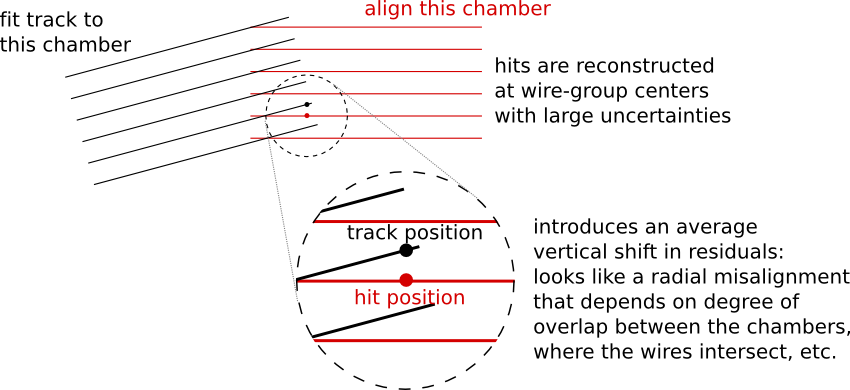
\includegraphics[width=\linewidth]{vertical_residual.png}

\vfill
\scriptsize
\begin{itemize}
\item Effect would be cleanest in beam-halo, where tracks are
  parallel to the beam and you can see the individual wires
\item They're smeared in cosmic ray data, but this bias can still be
  present in the mean
\end{itemize}
\end{frame}

\begin{frame}
\frametitle{MC study}
\scriptsize
\begin{itemize}
\item Beam-halo MC, perfect alignment
\item Black: track fitted to reference chamber, extrapolated to target chamber
\item Red: hit in target chamber
\item Wires intersect near the middle of the overlap region, making the average residual zero
\item Second plot: apply a cut to change the degree of overlap.
  (Region of overlap is much larger in data because segment-matching
  was more inclusive: tracks in MC sample are full standAloneMuons,
  crossing multiple stations, our CRUZET tracks are pairs of segments)
\end{itemize}

\vfill
\begin{columns}
\column{0.5\linewidth}
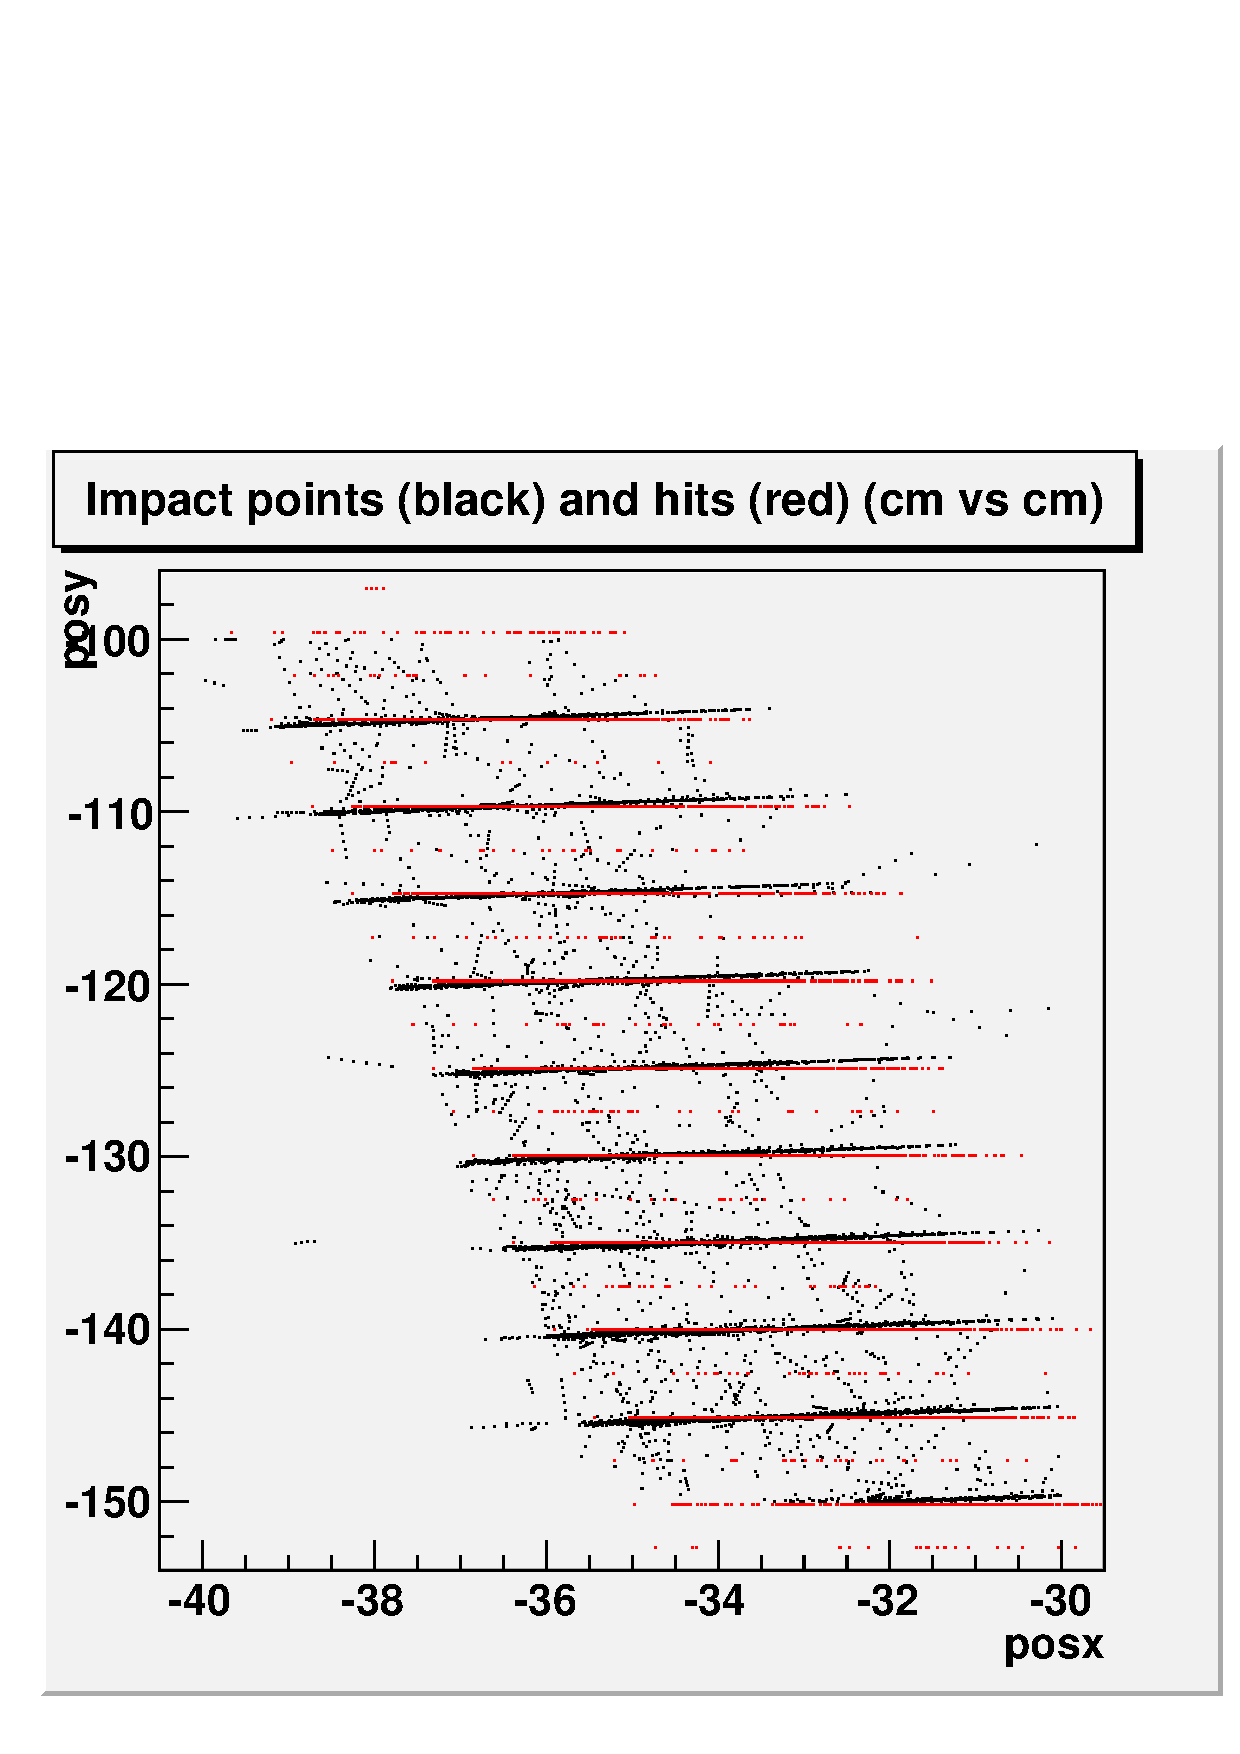
\includegraphics[width=\linewidth]{selectioneffect_nocut.pdf}
\column{0.5\linewidth}
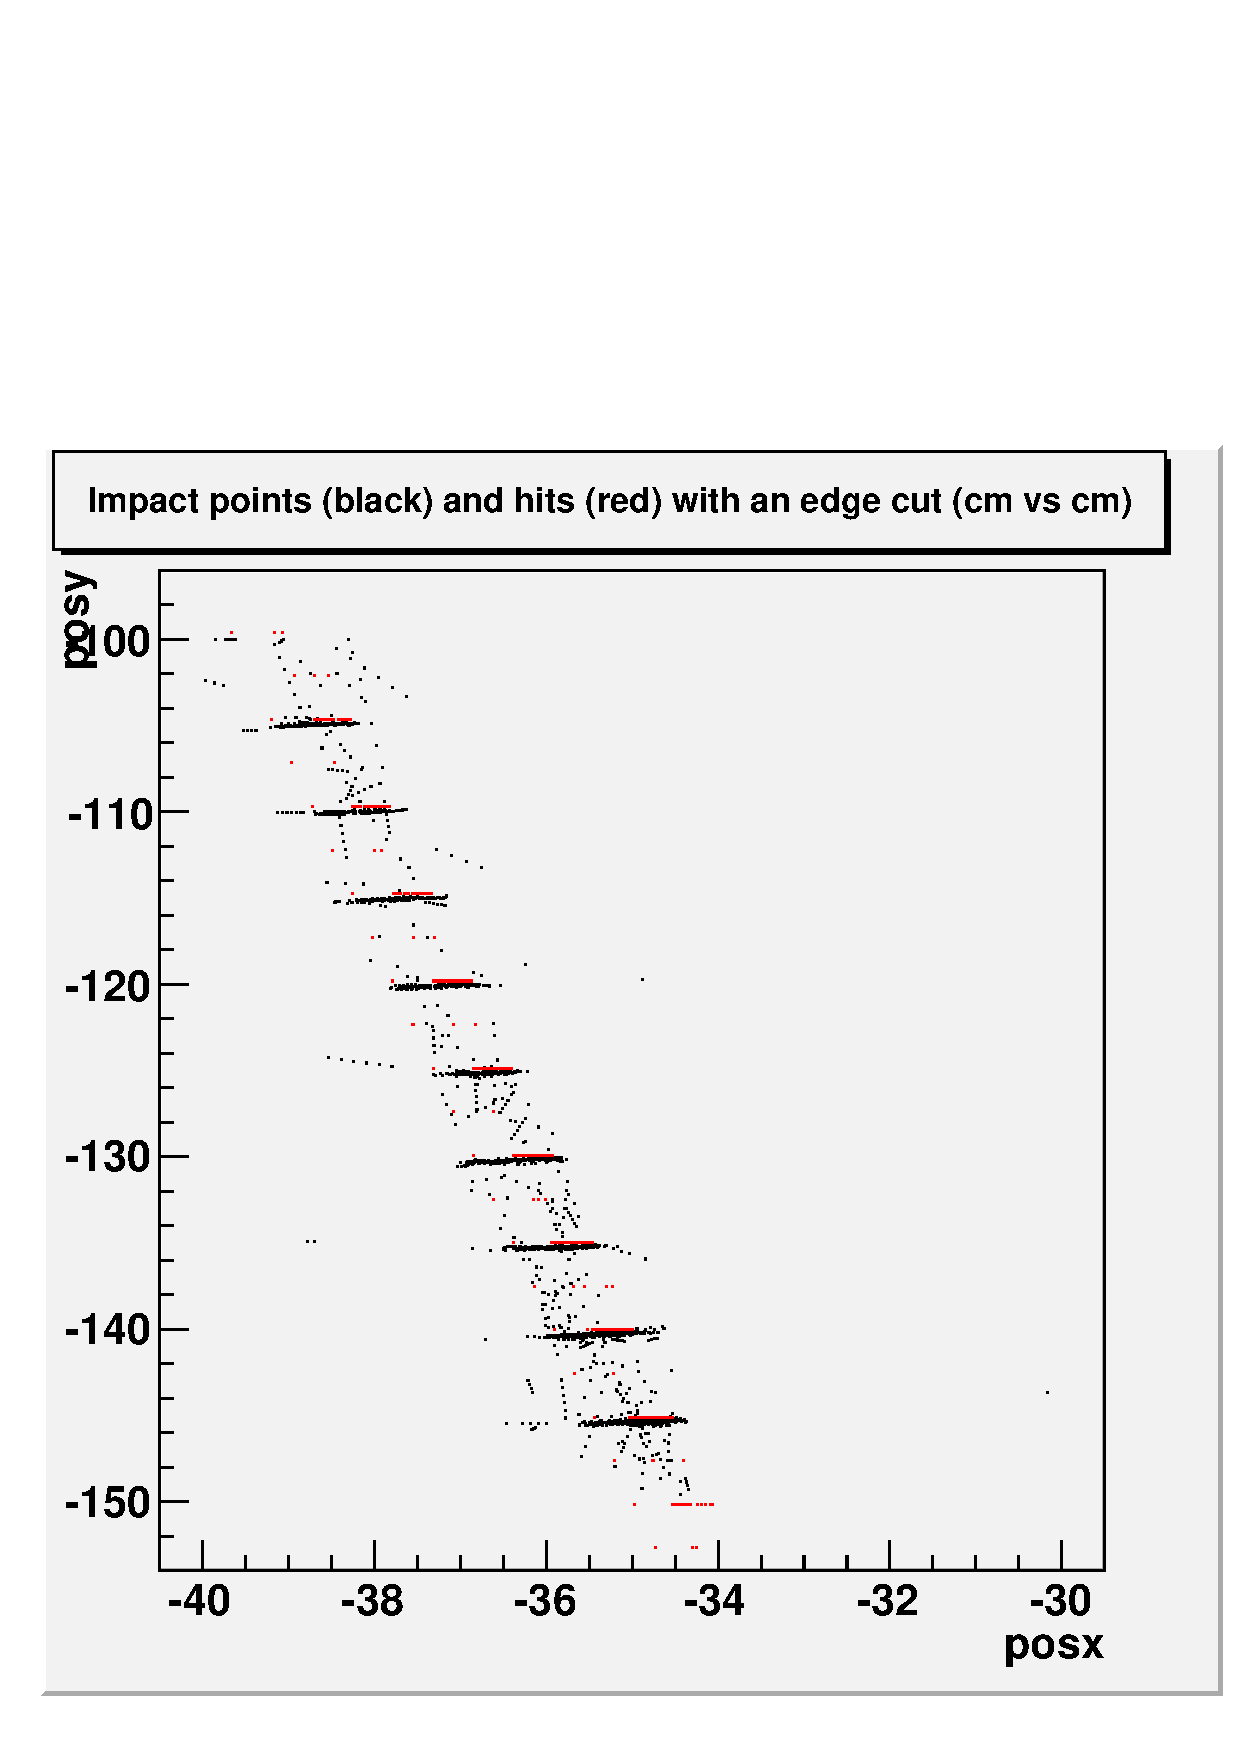
\includegraphics[width=\linewidth]{selectioneffect_withcut.pdf}
\end{columns}
\end{frame}

\begin{frame}
\frametitle{$y$-residuals}
\scriptsize
\begin{itemize}
\item First plot: no cut, mean is 50~microns
\item Second plot: same cut as previous page, mean is -1.7~mm
\item Third plot: cut in the opposite direction, simulating the track-reconstruction used in data, mean is 6.0~mm
\item These distributions are much broader in cosmic rays, but might have the same mean-shift
\end{itemize}

\vfill
\begin{columns}
\column{0.35\linewidth}
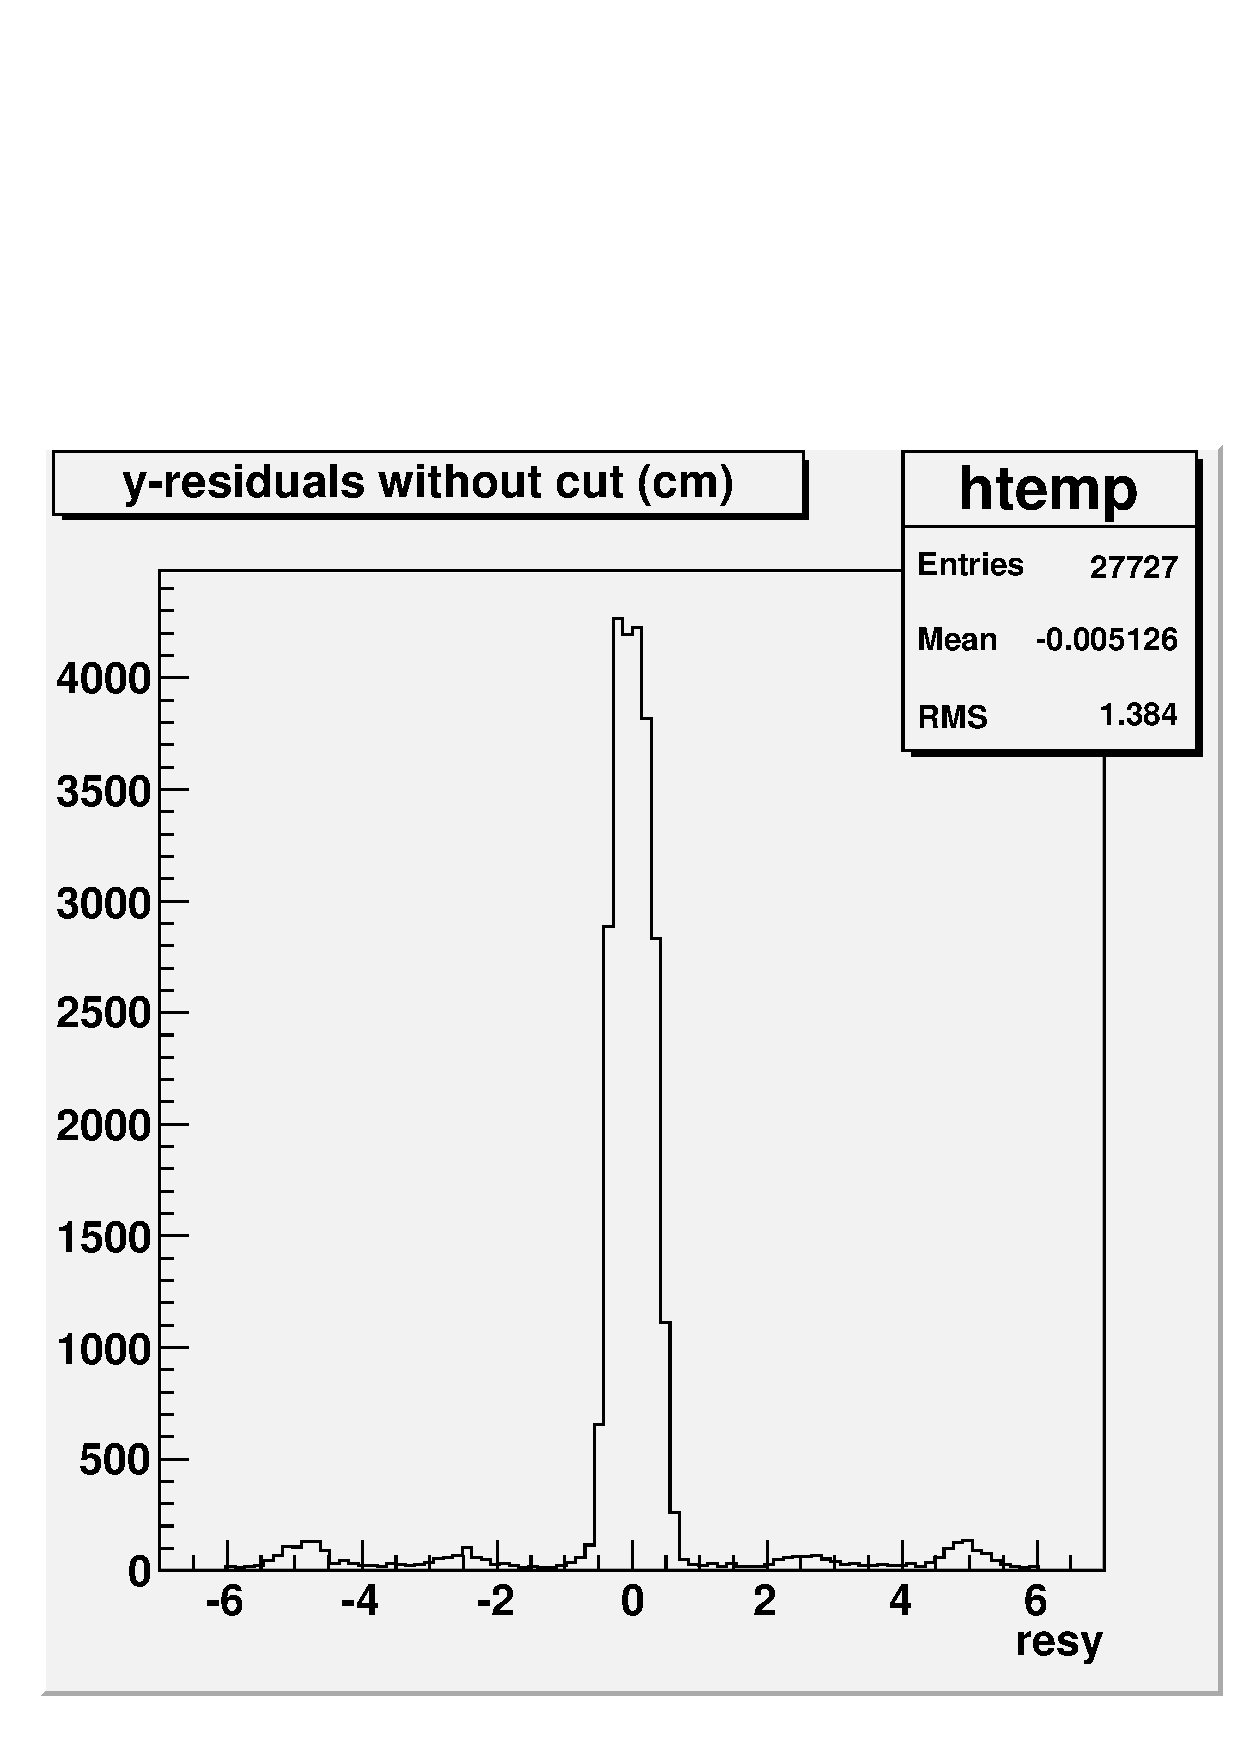
\includegraphics[width=\linewidth]{selectioneffect_resid_nocut.pdf}
\column{0.35\linewidth}
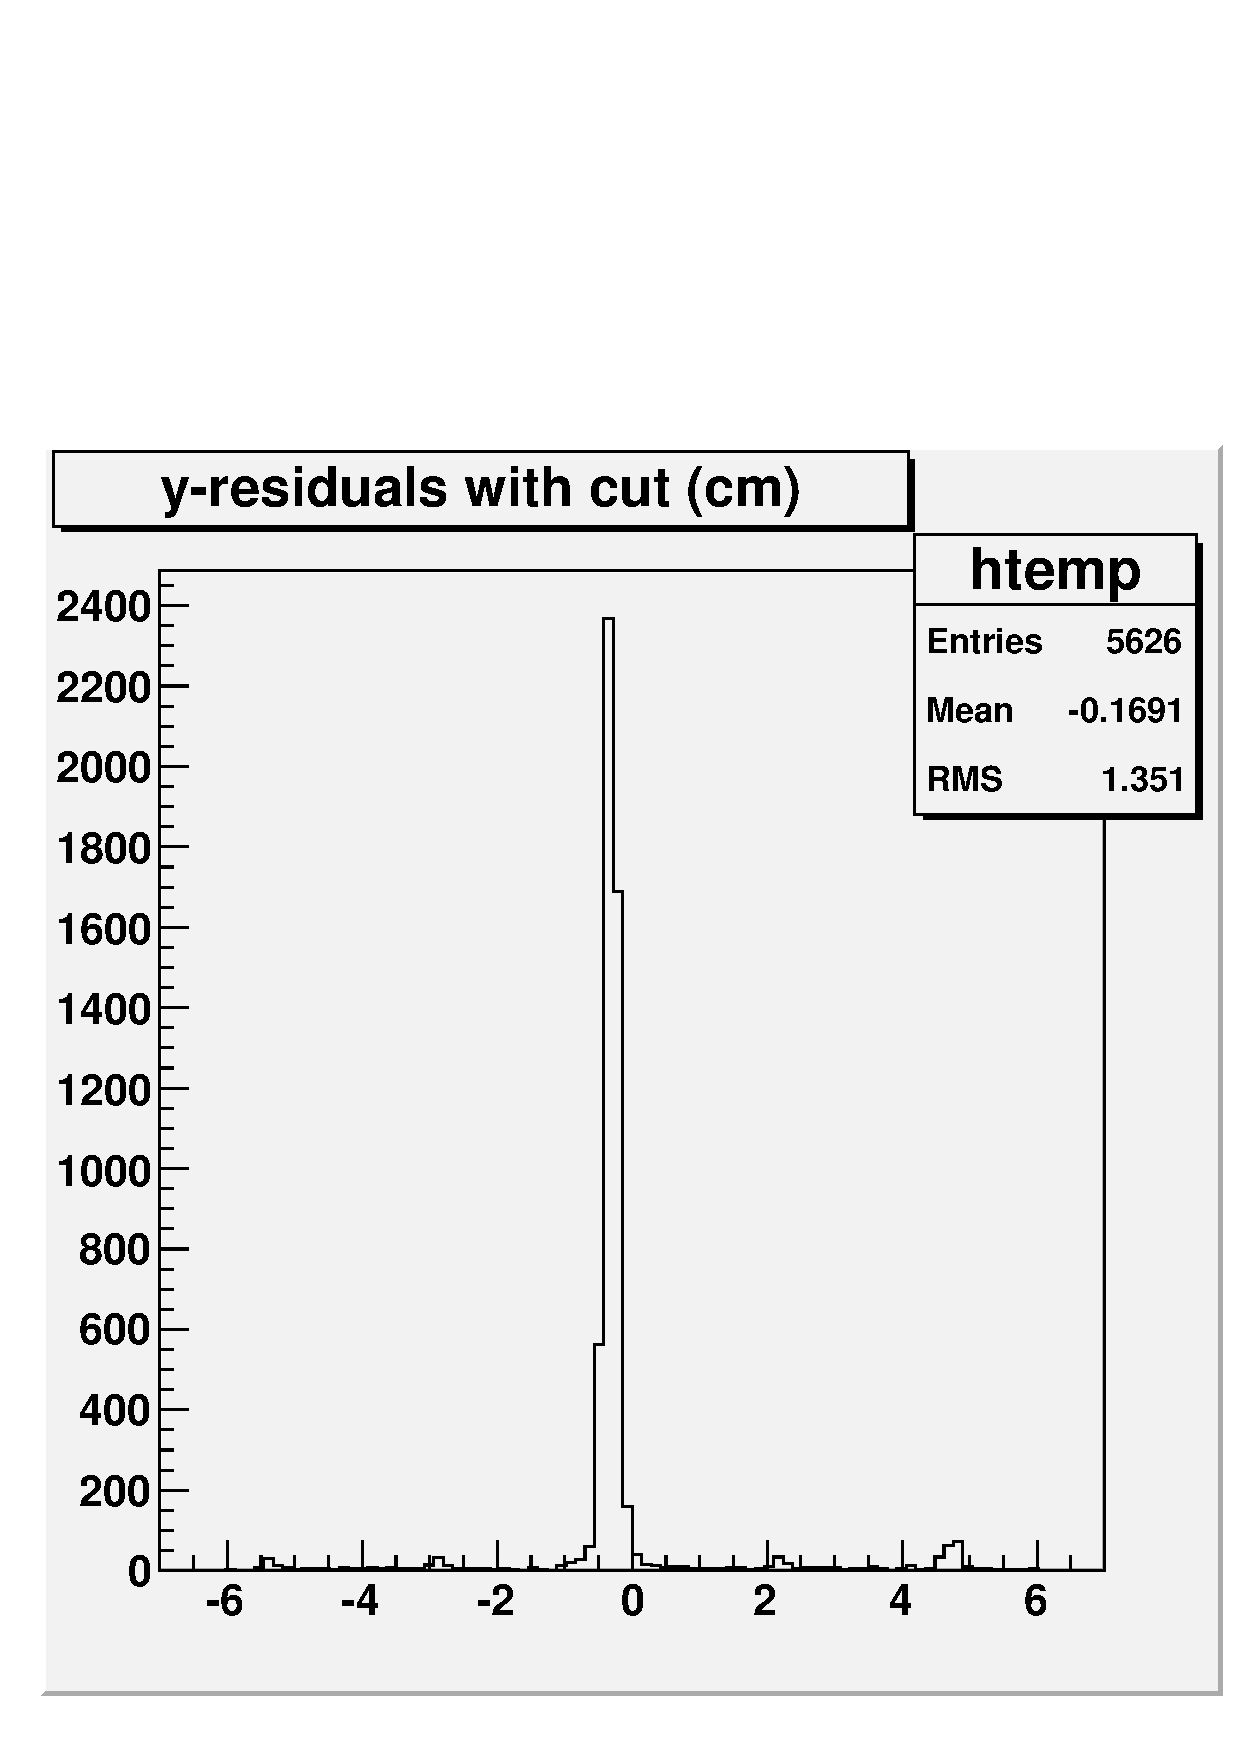
\includegraphics[width=\linewidth]{selectioneffect_resid_withcut.pdf}
\column{0.35\linewidth}
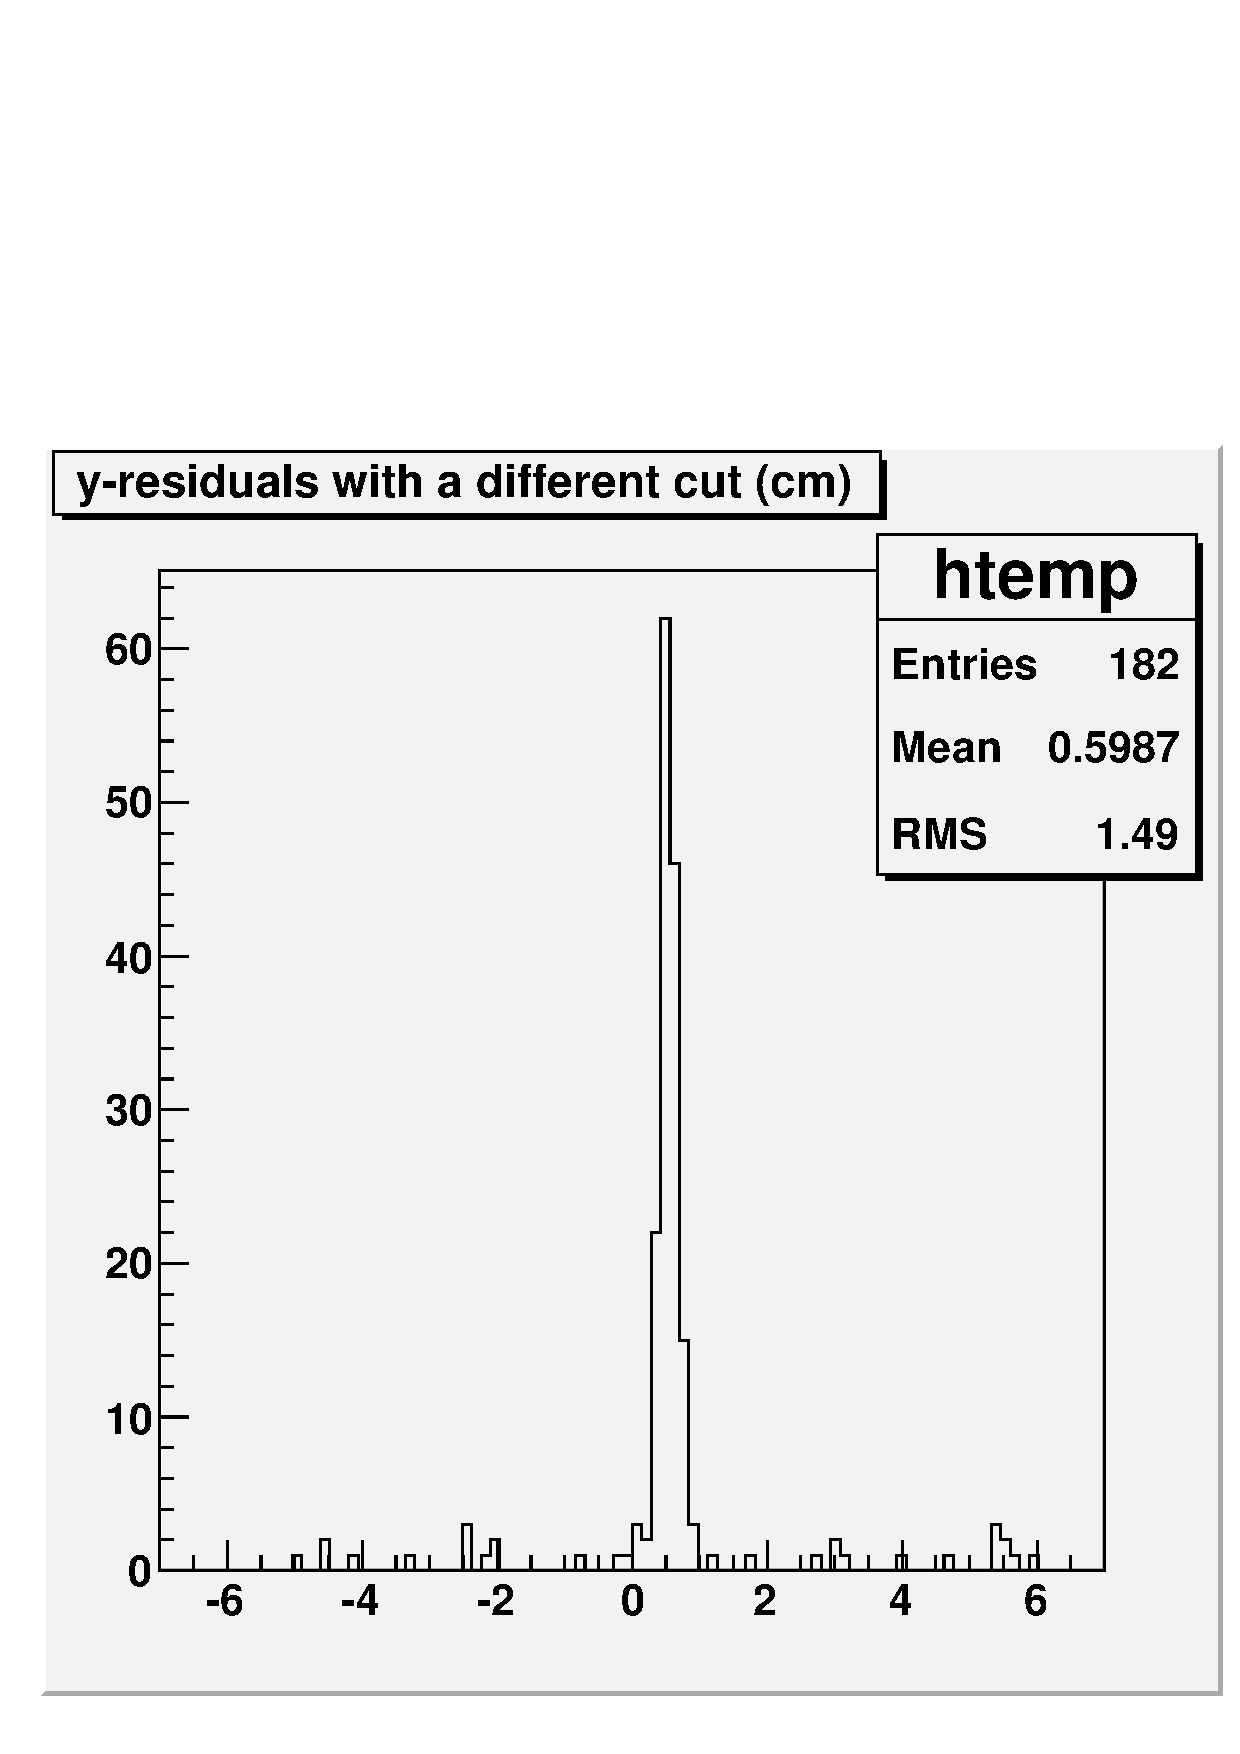
\includegraphics[width=\linewidth]{selectioneffect_resid_withanothercut.pdf}
\end{columns}
\label{numpages}
\end{frame}

\end{document}
